\documentclass[11pt]{article}
\usepackage[utf8]{inputenc}
\usepackage[letterpaper, total={6in, 9in}]{geometry}
\usepackage[table,xcdraw]{xcolor}
\usepackage{hyperref}
\usepackage{adjustbox,lipsum}

\usepackage{booktabs}
\usepackage{float}
\usepackage{tabularx}
\usepackage{hyperref}
\hypersetup{
    colorlinks,
    citecolor=black,
    filecolor=black,
    linkcolor=red,
    urlcolor=blue
}
\usepackage[round]{natbib}

\graphicspath{ {Assets/} }

\title{SE 3XA3: Software Requirements Specification\\Sudoku Solver}

\author{Team 08, SudoCrew
		\\ Rashad A. Bhuiyan (bhuiyr2)
		\\ Kai Zhu (zhuk2)
		\\ Stanley Chan (chans67)
}

\date{\today}

\begin{document}

\maketitle

\pagenumbering{roman}
\tableofcontents
\listoftables
\listoffigures

\begin{table}[bp]
\caption{\bf Revision History}
\begin{tabularx}{\textwidth}{p{3cm}p{2cm}X}
\toprule {\bf Date} & {\bf Version} & {\bf Notes}\\
\midrule
2022-02-07 & 1.0 & Initalized document with SRS structure\\
Date 2 & 1.1 & Notes\\
\bottomrule
\end{tabularx}
\end{table}

\newpage

\pagenumbering{arabic}

This document describes the requirements for a Sudoku Solver.  The template for the Software
Requirements Specification (SRS) is a subset of the Volere
template~\citep{RobertsonAndRobertson2012}.  If you make further modifications
to the template, you should explicity state what modifications were made.

\section{Project Drivers}

\subsection{The Purpose of the Project}
The purpose of this software application is to provide a comprehensive suite of tools for generating, recognizing, and solving Sudoku puzzles. The application will provide a web-based front-end with an intuitive interface to cater to users of different technical abilities on most modern hardware. Computer vision is also utilized to improve ease of use, by directly interfacing puzzles from print-media to the application.

\subsection{The Stakeholders}
\subsubsection{The Client}
The client of the project are the instructor, Dr. Asghar Bokhari, and teaching assistants of SFWRENG 3XA3. The clients stipulate the content and deadlines of the deliverables.

\subsubsection{The Customers}
The customers are any individuals with an interest in Sudoku. These includes hobbyists who seek to play the game or verify their solutions. The application is suitable for all demographics who can operate a web browser.

\subsubsection{Other Stakeholders}
Other stakeholders of the project include math teachers who may print generated puzzles from the application to use in educational setting. Tim Ruscica, the original developer of the open source Sudoku GUI Solver upon which this project is based on, also has a stake in seeing the expansion of features that stem from his work. Additionally, members of the SudoCrew development team are also stakeholders responsible for implementing and testing the application.

\subsection{Mandated Constraints}
\subsubsection{Solution Design Constraints}
\textbf{Description}: The game must operate on any browser with JavaScript enabled.
\\
\textbf{Rationale}: Potential users of the game will have access to a browser that can render JavaScript elements.
\\
\textbf{Fit Criterion}: The game will be made to operate on any browser with JavaScript enabled.

\subsubsection{Implementation Environment of the Current System}
N/A

\subsubsection{Partner or Collaborative Applications}
There are two main libraries used in the program; Flask and OpenCV. OpenCV is an API that allows for image recognition while Flask is a web framework that allows developers to build web applications.

\subsubsection{Off-the-Shelf Software}
N/A

\subsubsection{Anticipated Workplace Environment}
The Internet with PC, laptop, mobile device, or tablet as a browsing device.

\subsubsection{Schedule Constraints}
\textbf{Description}: The project must follow the project schedule shown in the Tasks section.
\\
\textbf{Rationale}: The project must follow a predetermined plan in order to meet deliverable due dates on time.
\\
\textbf{Fit Criterion}: The project will follow the project schedule shown in the Tasks section.

\subsubsection{Budget Constraints}
N/A

\subsubsection{Enterprise Constraints}
N/A

\subsection{Naming Conventions and Terminology}
\begin{table}[H]
\caption{\bf Table of Naming Conventions and Terminology}
\centering
\begin{tabularx}{\textwidth}{p{3cm}X}
\toprule
Terminology     & Meaning \\
\midrule
UI     & User interface, the interface that allows for user interaction with the system. \\
Python & Language used for backend and frontend implementation through Flask.\\
HTML & Hypertext markup language, used to build websheets for the frontend part of the web application.\\
CSS & Cascading style sheets, used to style HTML files to make the application look more appealing.\\
JavaScript & Primary language used for scripting and functionality of the web application. \\
Git & The primary system for version control and code collaboration.\\
OpenCV & An open source computer vision library, and serves as the main Python library that will be used to detect Sudoku boards. \\
Pytest & A Python library designed to help create tests for Python code. \\
Pydoc & A Python library used to generate documentation for Python code. \\
Flask & A micro web framework for Python, and will mainly be used to create our web application and handle requests from the web.\\
\bottomrule
\end{tabularx}
\end{table}
\subsection{Relevant Facts and Assumptions}

\subsubsection{Facts}

\begin{enumerate}
    \item The original repository for the existing Sudoku solver has approximately 400 lines of code spread across 3 Python files.
    \item The existing Sudoku solver solves hardcoded Sudoku boards and displays the solution in the command line.
\end{enumerate}

\subsubsection{Assumptions}

\begin{enumerate}
    \item The user has a stable Internet connection to use the web application.
    \item The Sudoku board uploaded is a 9x9 Sudoku board.
\end{enumerate}

\section{Functional Requirements}

\subsection{The Scope of the Work and the Product}

\subsubsection{The Context of the Work}
\begin{figure}[H]
    \centering
    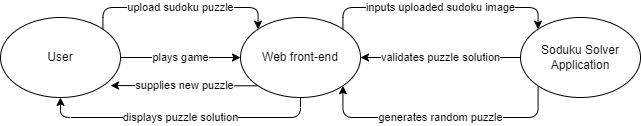
\includegraphics[width=\textwidth]{sudoku_scope}
    \caption{Work Context Diagram: The user either uploads a manually inputted or photographed Sudoku to receive feedback on a valid solution, or plays the game on a randomly generated puzzle grid. The Web front-end handles user input and interactive game-play while passing and receiving solution data to the back-end solver application.}
    \label{fig:my_label}
\end{figure}

\subsubsection{Work Partitioning}
\begin{table}[H]
\caption{\bf Table of Work Partitioning Events}
\label{tab:my-table}
\resizebox{\textwidth}{!}{%
\begin{tabular}{|c|l|l|l|}
\hline
\textbf{Event Number} & \multicolumn{1}{c|}{\textbf{Event Name}} & \multicolumn{1}{c|}{\textbf{Input}} & \multicolumn{1}{c|}{\textbf{Output}} \\ \hline
1 & Arrives at Homepage     & Mouse          & Webpage Generation   \\ \hline
2 & Uploading a sudoku board through an image     & Mouse          & Sudoku Board Solution   \\ \hline
3 & Uploading a sudoku board through manual input & Keyboard/Mouse & Sudoku Board Solution   \\ \hline
4 & Start a game of Sudoku                        & Mouse          & Sudoku Board Generation \\ \hline
\end{tabular}%
}
\end{table}

\subsubsection{Individual Product Use Cases}

\subsection{Functional Requirements}

\begin{enumerate}
    \item [BE1.] The user arrives at the main application portal (homepage)
    \begin{enumerate}
        \item [FR1.] The system must display links to play or get solution for a Sudoku game.
        \item [FR2.] The system shall display options for manual input or photo upload for the Sudoku solver.
        \item [FR3.] The system shall display an error if user browser is incompatible with the application.
    \end{enumerate}
    \item [BE2.] The user uploads a Sudoku board through an image
    \begin{enumerate}
        \item [FR4.] The system shall display a loading indicator to the user to show that their picture is being uploaded and solved.
        \item [FR5.] The system shall attempt to interpret the uploaded picture as a 9x9 Sudoku board modelled as an array.
        \item [FR6.] If the system fails to interpret a 9x9 Sudoku board from the uploaded image, the system shall inform the user that the picture could not be interpreted.
        \item [FR7.] The system shall input the 9x9 array into the Sudoku solver algorithm to solve the Sudoku board.
        \item [FR8.] If the system finds a solution to the Sudoku board, the system shall display the solution in the user interface.
        \item [FR9.] If the system does not find a solution, the system shall notify the user that the Sudoku board is invalid.
    \end{enumerate}
    \item [BE3.] The user uploads a Sudoku board through manual input
    \begin{enumerate}
        \item [FR10.] The system should display a loading indicator to inform the user that the Sudoku board is being solved.
        \item [FR11.] The system should use the Sudoku solver algorithm to solve the inputted Sudoku board.
        \item [FR12.] If the system fails to find a solution to the Sudoku board, the system should inform the user that the Sudoku board is invalid.
        \item [FR13.] If the system finds a solution, the system should display the solution to the user through the user interface.
    \end{enumerate}
    \item [BE4.] The user starts a game of Sudoku
    \begin{enumerate}
        \item [FR14.] The system should generate a random valid Sudoku board.
        \item [FR15.] The system should output the generated Sudoku board to the user through the user interface.
    \end{enumerate}
\end{enumerate}

\section{Non-functional Requirements}

\subsection{Look and Feel Requirements}

\subsection{Usability and Humanity Requirements}

\subsection{Performance Requirements}

\subsection{Operational and Environmental Requirements}

\subsection{Maintainability and Support Requirements}

\subsection{Security Requirements}

\subsection{Cultural Requirements}

\subsection{Legal Requirements}

\subsection{Health and Safety Requirements}

This section is not in the original Volere template, but health and safety are
issues that should be considered for every engineering project.

\section{Project Issues}

\subsection{Open Issues}

\subsection{Off-the-Shelf Solutions}

\subsection{New Problems}

\subsection{Tasks}

\subsection{Migration to the New Product}

\subsection{Risks}

\subsection{Costs}

\subsection{User Documentation and Training}

\subsection{Waiting Room}

\subsection{Ideas for Solutions}

\bibliographystyle{plainnat}

\bibliography{SRS}

\newpage

\section{Appendix}

This section has been added to the Volere template.  This is where you can place
additional information.

\subsection{Symbolic Parameters}

The definition of the requirements will likely call for SYMBOLIC\_CONSTANTS.
Their values are defined in this section for easy maintenance.


\end{document}
